\section {Conclusions}

Gaseous adsorption on solid surfaces has been extensively studied over the past few decades with much learned about how molecular geometry and orientation of the adsorbate are influenced by the proximity of the solid slab.  For a liquid surface where the surface slab is no longer rigid but has molecules with considerable freedom of movement, the surface and approaching gas molecules can be active partners in attaining the optimal geometry and orientation necessary for adsorption and subsequent uptake.    And unlike the solid surface defined by a sharp plane, the interfacial region for the liquid-gas system is much broader, extends on either side of a defined center plane, and is host to a broad distribution of gas-liquid molecular geometries and orientations that change as the gas molecules transit through the interfacial region into the bulk liquid.  Although  our current molecular level understanding of  the complex dances that these molecules play in this fluid interfacial region is in its infancy, emerging studies such as these are beginning to provide unique new insights that are key to understanding many  environmentally important processes at aqueous surfaces.

Presented herein are the results of several classical molecular dynamic simulations that focus on understanding how surface water molecules and adsorbing \suldiox~gas molecules twist and turn as the gas transits the interfacial region. The computational studies emulate and expand on the experimental spectroscopic studies from this laboratory which have found \suldiox~surface complexation at a water surface.\cite{Tarbuck2005,Tarbuck2006,Ota2011}  These spectroscopic studies show clear evidence of \suldiox-water surface complexation but details about this surface complex could only be inferred from spectral changes in the surface water spectrum since \suldiox~could not be monitored directly.   These simulations do not have that limitation and hence can provide information about the behavior of both surface partners and in particular, how their proximity influences the orientation behavior of each other.  The orientational information obtained in these simulations are provided via calculated depth profiles which show the molecular distribution of orientations of the two different interfacial molecules throughout the dimensions of the interfacial region.

The simulations described herein show that gaseous \suldiox~quickly adsorbs to the water surface and continues to bind until a complete surface coverage is reached. Surface waters reorient in the presence of adsorbed \suldiox. The waters at the interface of a neat-water surface tend to lay flatter to the surface than when a saturating layer of \suldiox~is present. The waters interacting with the layer of adsorbed \suldiox~orient more perpendicularly to the interface, and further expose their ``free-OH'' uncoupled bonds for interactions with \suldiox, and hydrate complex formation. Furthermore, we have found that surface waters underneath a blanket layer of adsorbed \suldiox~will penetrate further into the gas phase, allowing for greater mobility of waters away from the aqueous bulk in the presence of \suldiox.

Through these simulations we characterize the orientational behavior of \suldiox~during and after adsorption. Our equilibrium neat-water simulations show that a single \suldiox~molecule, representing a low concentration, has a high surface affinity. At a high \suldiox~concentration in the saturated systems, \suldiox~molecules are also surface active, and are found further out of the water phase than at the lower concentration. These \suldiox~form a bound layer of molecules that crowd the surface and interact with the surface waters. The orientation of \suldiox~on the water surface was found to be similar for both low and high concentrations. Those \suldiox~molecules at or below the surface strongly orient with the sulfur atom pointed in towards the water bulk, and the oxygen atoms out towards the gas phase. The \suldiox~slightly above the water surface loses the orientational preference within 10 $\AA$ and those further from the water are more isotropically oriented. Figure \ref{fig:so2-surface-cartoon} depicts what the neat-water and saturated surfaces might look like for both \suldiox~and \wat~orientations and locations.

\begin{figure}[h!]
	\begin{center}
		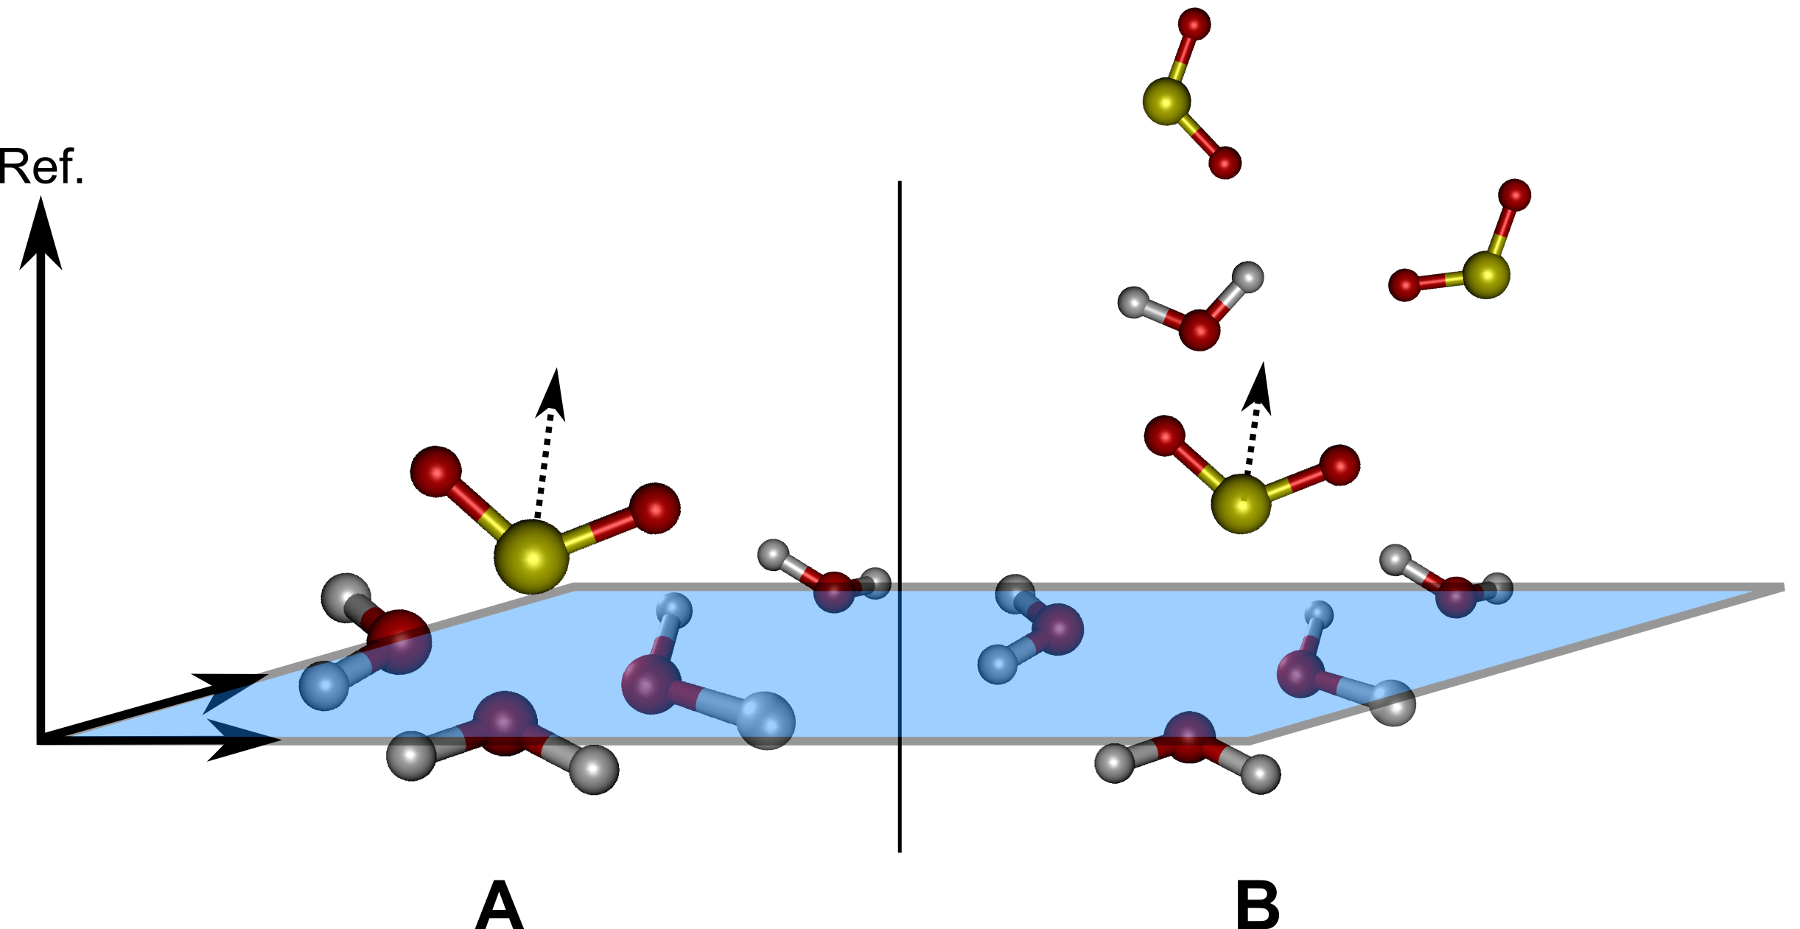
\includegraphics[scale=1.0]{images/angle-cartoons/system-surface.png}
		\caption{\wat~and \suldiox~both exhibit preferred orientations in the region near the liquid-gas interface. The neat-water system (A) with a single \suldiox~molecule (low-concentration) has surface waters orienting mostly flat to the interface. When the \suldiox~concentration is increased, as in the saturated system (B), the waters at the surface behave similar to the neat-water interface, but waters that venture into the adsorbed \suldiox~gas layer orient strongly with their bisectors pointing out from the aqueous phase towards the gas. In both cases, the \suldiox~orients with its molecular bisector pointing out to the gas phase when it is near the surface, and isotropically further into the gas phase. Sulfur, oxygen and hydrogen atoms are colored yellow, red, and white, respectively.}
		\label{fig:so2-surface-cartoon}
	\end{center}
\end{figure}

Steered molecular dynamics simulations were used to model the behavior of an adsorbing \suldiox~as it moves from the gas phase above the water down through the surface and into the bulk. The results for the transit through the interface show that in both systems of low and high \suldiox~concentration an adsorbing \suldiox~has very similar orientation to those already bound to the water surface. The \suldiox~reorients as it makes its first contact with the water interface. Within 5 $\AA$ of the surface the \suldiox~is mostly oriented with its sulfur towards the water phase. The \suldiox~pulled further into the water bulk retains its orientation until it is past the interfacial region and then isotropically orients with the bulk water.

Having now examined the transition of \suldiox~from the gas to adsorbed aqueous phases, we are better able to research the many questions remaining of adsorption and interfacial chemistry of gas molecules. What species form during the adsorption transition, and how do molecular properties affect the process? Can we form a theory that will more fully explain the transit of many small molecules of environmental and industrial interest? This study is one of several characterizing \suldiox~adsorption and behavior on aqueous surfaces. We plan to report further results of ongoing computational simulation and experimental studies regarding temperature and chemical constituent effects on atmospherically relevant water surfaces.
